\documentclass[conference]{IEEEtran}
\IEEEoverridecommandlockouts

\usepackage[T1]{fontenc}
\usepackage[utf8]{inputenc}
\usepackage{microtype}
\setlength{\emergencystretch}{2em}
\usepackage{amsmath,amssymb,amsfonts,bm}
\usepackage{graphicx}
\usepackage{booktabs}
\usepackage{multirow}
\usepackage{tabularx}
\usepackage{xcolor}
\usepackage{tikz}
\usetikzlibrary{arrows.meta,positioning,fit,calc}
\usepackage{algorithm}
\usepackage{algpseudocode}
\usepackage{cite}
\usepackage[inline]{enumitem}
\setlist{itemsep=1pt,topsep=3pt}
\usepackage[hidelinks]{hyperref}
\usepackage[capitalize,noabbrev]{cleveref}

\makeatletter
\newcommand{\tabinput}[1]{\@@input #1 }
\makeatother
\newcommand{\p}{\mathbf{p}}
\newcommand{\q}{\mathbf{q}}
\newcommand{\FK}{\mathrm{FK}}
\newcommand{\atantwo}{\operatorname{atan2}}
\newcommand{\code}[1]{\texttt{#1}}
\newcommand{\finding}[1]{\par\smallskip\noindent\textbf{Finding #1.}~}

\title{Learning Inverse Kinematics by Imitating a Numerical Solver: Analysis and Improvements on Two 3-DOF Manipulators}

\author{\IEEEauthorblockN{Durgesh S. Reddiyar}
\IEEEauthorblockA{Ira A. Fulton Schools of Engineering\\
Arizona State University, Tempe, AZ, USA\\
dreddiya@asu.edu}}

\begin{document}
\maketitle

\begin{abstract}
To move a robot arm's hand to a target, we need its inverse kinematics (IK): the joint values that place the hand there. A popular shortcut is to train a neural network for IK, using an existing numerical IK solver to create the training examples. This report studies such a system, built with the MATLAB Robotics Toolbox and Keras for two simple three-joint arms: an all-rotary (RRR) arm and a cylindrical (RPP) arm. Measured by how far the hand actually lands from the target, the baseline network misses by a median of about 4\% of the arm's reach, and by more than half the reach for the worst 5\% of targets. Keras's default ``accuracy'' metric gives this network 74\% and cannot reveal the problem, because it only checks which of the three joint values is largest. We trace most of the error to the training data. The solver often returns different, equally valid joint solutions for neighbouring targets, so the network is asked to learn an inconsistent mapping. The solver's failures come simply from targets outside the arm's reach. And one data generator confuses a position coordinate with an angle. Fixing the data makes the network $43\times$ more accurate at the median and about $200\times$ more accurate on the hardest targets. The fixes are to always use the same solution branch, to compute exact labels, and to predict the sine and cosine of each angle. The improved network also makes a good starting guess for the numerical solver: it needs $3.5\times$ fewer iterations and always returns the intended solution. We release the code and summarise the lessons as a short checklist.
\end{abstract}

\begin{IEEEkeywords}
Inverse kinematics, neural networks, robot manipulators, Levenberg--Marquardt, reproducibility, evaluation metrics.
\end{IEEEkeywords}

\section{Introduction}
\label{sec:intro}

Inverse kinematics asks for joint variables $\q$ that place a manipulator's end effector at a desired pose. For most serial arms, the forward map $\p=\FK(\q)$ is a closed-form composition of homogeneous transforms~\cite{denavit1955kinematic,siciliano2009robotics}. Its inverse, however, is a set-valued map: a target can have no solution, a finite number of them, or a continuum. Classical treatment splits into analytic solutions for special geometries~\cite{pieper1968kinematics,raghavan1993inverse,diankov2010automated} and iterative Jacobian methods for the general case~\cite{wampler1986manipulator,nakamura1986inverse,buss2004introduction,sugihara2011solvability,beeson2015trac}.

Learning the inverse map with a neural network is a long-standing idea~\cite{guez1988solution,jordan1992forward,dsouza2001learning,oyama2001modular,bocsi2011learning,csiszar2017solving}. A trained network gives an answer in a single, constant-time forward pass. Universal-approximation results~\cite{hornik1989multilayer} make it tempting to treat IK as plain regression. It has been known since at least Jordan and Rumelhart~\cite{jordan1992forward} that this view is incomplete. When the target relation is one-to-many, a least-squares regressor averages solutions that may not themselves be solutions. Recent work addresses multiplicity explicitly through structured prediction~\cite{bocsi2011learning}, mixture or generative models~\cite{bishop1994mixture,ardizzone2019analyzing,ames2022ikflow}, or by partitioning the data~\cite{csiszar2017solving}.

Despite this literature, a very common first implementation of ``IK with a neural network'' consists of four steps:
\begin{enumerate*}[label=(\arabic*)]
\item sample random Cartesian targets;
\item label them by running an off-the-shelf numerical solver;
\item fit an MLP with a stock deep-learning API; and
\item report the API's default metric together with a few qualitative comparisons.
\end{enumerate*}
This report presents such a pipeline, developed at Arizona State University for two textbook 3-DOF arms~\cite{siciliano2009robotics} using Peter Corke's Robotics Toolbox for MATLAB~\cite{corke1996toolbox,corke2017rvc} and Keras/TensorFlow~\cite{chollet2015keras,abadi2016tensorflow}.

We describe the pipeline in full, evaluate it in task space, identify what limits its accuracy, and show how to fix it. The pitfalls we find, an uninformative default metric and inconsistent training labels, are common well beyond this project~\cite{pineau2021improving,kapoor2023leakage}.

\paragraph{Contributions}
\begin{itemize}
\item \textbf{A complete description of the baseline pipeline} (\cref{sec:pipeline}). This includes the network architecture, loss, optimiser, and training split, all taken directly from the saved models and code.
\item \textbf{An analysis of the data, the metric, and the evaluation} (\cref{sec:audit}). It identifies the causes of the baseline's error summarised in the abstract.
\item \textbf{A task-space evaluation} of all seven trained models (\cref{sec:reeval}), including generalisation gaps and failure geometry.
\item \textbf{A controlled study} (\cref{sec:study}) that keeps the inputs fixed and isolates the effects of label consistency, angle wrapping, loss, output representation, and data scale. It also covers a hybrid learned-warm-start solver and latency measurements.
\item \textbf{A practical checklist} (\cref{sec:discussion}) and a self-contained release of the analysis code.
\end{itemize}

\section{Background and Related Work}
\label{sec:related}

\paragraph{Numerical IK}
Iterative methods linearise $\FK$ around the current estimate and solve for a joint update. The undamped pseudo-inverse step is ill-conditioned near singular configurations. Damped least squares~\cite{wampler1986manipulator,nakamura1986inverse} and its adaptive form, the Levenberg--Marquardt (LM) method~\cite{levenberg1944method,marquardt1963algorithm,sugihara2011solvability}, trade step accuracy for robustness. The Robotics Toolbox (RTB) \code{ikine} used here implements an LM scheme with a multiplicatively adapted damping factor~\cite{corke2017rvc}. Production libraries such as TRAC-IK~\cite{beeson2015trac} add random restarts and joint-limit handling. Two properties of all local methods matter for this paper. First, the solution they return depends on the initial guess, i.e.\ on which basin of attraction the guess falls into. Second, joint angles are accumulated without wrapping, so a returned angle is only defined up to multiples of $2\pi$.

\paragraph{Analytic IK}
Arms whose last three axes intersect, and the two 3-DOF arms studied here, admit closed-form solutions~\cite{pieper1968kinematics,siciliano2009robotics}. IKFast generates such solvers automatically~\cite{diankov2010automated}. When an analytic solution exists, a learned model is redundant as a \emph{solver}. Such arms remain valuable as \emph{testbeds}, however, because exact ground truth and the full solution set are available. This is how we use them in \cref{sec:study}.

\paragraph{Learned IK}
Early neural IK work~\cite{guez1988solution} treated the inverse as direct regression. Jordan and Rumelhart~\cite{jordan1992forward} showed that, for non-convex inverse sets, direct inverse modelling converges to averages of valid solutions that are not solutions themselves. Their \emph{distal teacher} instead trains through a forward model. Later work localised the problem with local linear models~\cite{dsouza2001learning}, modular experts~\cite{oyama2001modular}, structured output learning~\cite{bocsi2011learning}, heuristic splitting of the dataset~\cite{csiszar2017solving}, or explicit conditional densities via mixture density networks~\cite{bishop1994mixture}, invertible networks~\cite{ardizzone2019analyzing}, and normalising flows~\cite{ames2022ikflow}. Output parameterisation also matters: angle outputs are discontinuous at the wrap point, and continuous embeddings such as $(\cos\theta,\sin\theta)$ are preferable~\cite{zhou2019continuity}.

\paragraph{Reproducibility}
Reproducibility programmes~\cite{pineau2021improving} and studies of data leakage in ML-based science~\cite{kapoor2023leakage} document how evaluation errors, especially train/test contamination and inappropriate metrics, can distort reported performance. IK is a convenient setting in which to study such effects, because exact ground truth makes their size measurable.

\section{Problem Setup}
\label{sec:setup}

Both manipulators are taken verbatim from the project code and use standard Denavit--Hartenberg (DH) conventions~\cite{denavit1955kinematic}. We use the convention of RTB's \code{Link([theta d a alpha sigma])}. Lengths are in the toolbox's unitless ``length units'' (LU).

\paragraph{Anthropomorphic RRR arm}
The DH parameters are $(a_i,\alpha_i,d_i)=(0,\pi/2,0)$, $(a_2,0,0)$, and $(a_3,0,0)$, with $a_2=a_3=10$~LU. The forward kinematics of the wrist point are
\begin{equation}
\label{eq:fk-rrr}
\p=\begin{bmatrix} c_1 r \\ s_1 r \\ a_2 s_2 + a_3 s_{23}\end{bmatrix},
\qquad r = a_2 c_2 + a_3 c_{23},
\end{equation}
where $c_i=\cos\theta_i$, $s_i=\sin\theta_i$, and $c_{23}=\cos(\theta_2+\theta_3)$. The workspace is the closed ball $\|\p\|\le a_2+a_3=20$. Away from singularities, every interior target has four solutions, indexed by a shoulder sign $\sigma_s\in\{\pm1\}$ and an elbow sign $\sigma_e\in\{\pm1\}$:
\begin{equation}
\label{eq:ik-rrr}
\begin{aligned}
\theta_1 &= \atantwo(p_y,p_x) + \tfrac{1-\sigma_s}{2}\pi,\\
c_3 &= \frac{\|\p\|^2-a_2^2-a_3^2}{2a_2a_3},\\
\theta_3 &= \atantwo\!\big(\sigma_e\sqrt{1-c_3^2},\,c_3\big),\\
\theta_2 &= \atantwo(p_z,\,\sigma_s\rho) - \atantwo(a_3 s_3,\,a_2 + a_3 c_3),
\end{aligned}
\end{equation}
with $\rho=\sqrt{p_x^2+p_y^2}$. The singular set consists of three parts:
\begin{itemize}
\item the $z$-axis, $\rho=0$ (shoulder singularity, where $\theta_1$ is undefined);
\item the boundary sphere, $\|\p\|=20$ (outstretched elbow, $\theta_3=0$);
\item the origin (folded elbow, $\theta_3=\pi$), which is reachable because $a_2=a_3$.
\end{itemize}

\paragraph{Cylindrical RPP arm}
The DH parameters are $(\theta_1, d_1{=}5, 0, 0)$ (revolute), $(0, d_2, 0, -\pi/2)$ (prismatic), and $(0, d_3, 0, 0)$ (prismatic). Hence
\begin{equation}
\label{eq:fk-rpp}
\begin{gathered}
\p = \big[-s_1 d_3,\; c_1 d_3,\; d_1 + d_2\big]^\top,\\
\theta_1 = \atantwo(-p_x,\,p_y),\quad d_2 = p_z - d_1,\quad d_3=\rho.
\end{gathered}
\end{equation}
With $d_3\ge0$, the solution is unique (up to $2\pi$ in $\theta_1$) except on the $z$-axis.

\paragraph{Metrics}
The quantity that matters for a positioning task is the \emph{task-space error} $e(\p)=\|\FK(\hat\q(\p))-\p\|$. Unlike joint-space error, it does not depend on which of several valid solutions a model returns, or on how angles are wrapped. We report its median, mean, and tail percentiles, and joint errors only after wrapping differences to $(-\pi,\pi]$.

\section{The Original Pipeline, As Implemented}
\label{sec:pipeline}

\Cref{fig:pipeline} summarises the system. The model and training details below are taken directly from the HDF5 model files, which store the full Keras model and training configuration (Keras~2.3.1, TensorFlow backend), and from \code{train.py}.

\begin{figure*}[t]
\centering
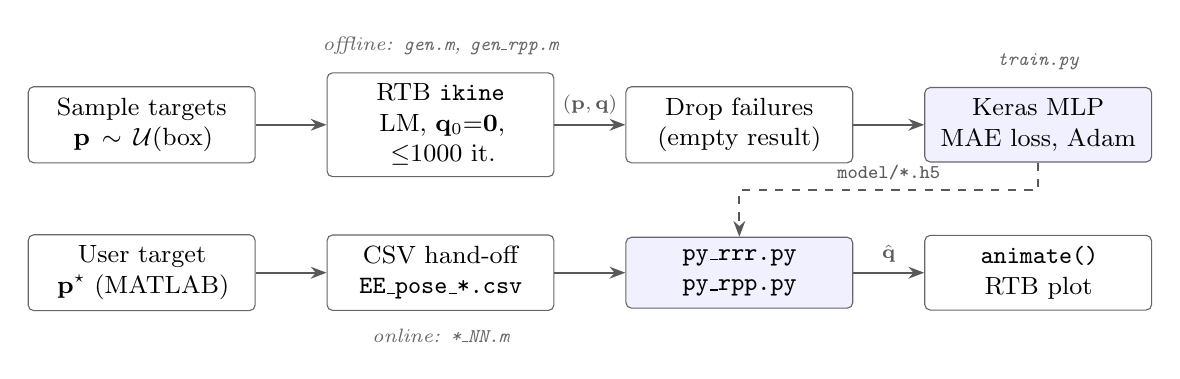
\begin{tikzpicture}[
  node distance=4mm and 9mm,
  box/.style={draw=black!60, rounded corners=2pt, align=center, font=\small, inner sep=4pt, minimum height=9mm, text width=26mm},
  hl/.style={box, fill=blue!6},
  ar/.style={-{Stealth[length=2mm]}, thick, black!65},
  lab/.style={font=\scriptsize\itshape, black!60}]
\node[box] (s) {Sample targets\\ $\p\sim\mathcal{U}(\text{box})$};
\node[box, right=of s] (ik) {RTB \code{ikine}\\ LM, $\q_0{=}\mathbf{0}$, $\le$1000 it.};
\node[box, right=of ik] (f) {Drop failures\\ (empty result)};
\node[hl, right=of f] (t) {Keras MLP\\ MAE loss, Adam};
\node[lab, above=1mm of ik] {offline: \code{gen.m}, \code{gen\_rpp.m}};
\node[lab, above=1mm of t] {\code{train.py}};
\draw[ar] (s) -- (ik); \draw[ar] (ik) -- node[above, font=\scriptsize]{$(\p,\q)$} (f); \draw[ar] (f) -- (t);
\node[box, below=9mm of s] (u) {User target\\ $\p^\star$ (MATLAB)};
\node[box, right=of u] (csv) {CSV hand-off\\ \code{EE\_pose\_*.csv}};
\node[hl, right=of csv] (py) {\code{py\_rrr.py}\\ \code{py\_rpp.py}};
\node[box, right=of py] (an) {\code{animate()}\\ RTB plot};
\node[lab, below=1mm of csv] {online: \code{*\_NN.m}};
\draw[ar] (u) -- (csv); \draw[ar] (csv) -- (py); \draw[ar] (py) -- node[above, font=\scriptsize]{$\hat\q$} (an);
\draw[ar, dashed] (t.south) -- ++(0,-3.5mm) -| node[pos=0.25, above, font=\scriptsize]{\code{model/*.h5}} (py.north);
\end{tikzpicture}
\caption{The original solver-supervised IK pipeline. Offline, random Cartesian targets are labelled by the Robotics Toolbox LM solver and an MLP is fitted to the successful pairs. Online, MATLAB passes a target to the network through CSV files and displays the arm with the Robotics Toolbox.}
\label{fig:pipeline}
\end{figure*}

\paragraph{Data generation (\code{gen.m}, \code{gen\_rpp.m})}
For the RRR arm, $10^4$ targets are drawn uniformly from the cube $[-15,15]^3$. Each target is passed, as a pure translation, to \code{SerialLink.ikine} with a position-only mask (\code{'mask',[1 1 1 0 0 0]}), the initial guess $\q_0=\mathbf{0}$, and \code{'ilimit',1000}. Targets for which the solver returns an empty result are dropped. For the RPP arm, the script draws $x\sim\mathcal{U}[\mathrm{deg2rad}(0),\mathrm{deg2rad}(360)]$ and $y,z\sim\mathcal{U}[5,200]$. We return to this choice in \cref{sec:audit-rpp}. An earlier dataset in the repository (\code{train\_rpp.csv}) used $x\sim\mathcal{U}[0,360]$ instead.

\paragraph{Model}
All production models share the architecture
\[
3\text{--}32\text{--}64\text{--}128\text{--}256\text{--}256_{\sigma}\text{--}256\text{--}128\text{--}128\text{--}64\text{--}3,
\]
with ReLU activations, one sigmoid layer (marked $\sigma$), a linear output, and 233{,}027 parameters. Training minimises the mean absolute error (MAE) with Adam~\cite{kingma2015adam} ($\eta=10^{-3}$, default moments) at batch size 768, with \code{metrics=['accuracy']}. Inputs and outputs are not normalised. The data are split 80:20 with \code{train\_test\_split(random\_state=1)}. The train/test gap in \cref{tab:models} matches this split to a recorded training run. The RRR model was checkpointed after 2k (smaller architecture), 10k, 15k, and 20k epochs; the 20k-epoch model ships with the demo.

\paragraph{Deployment}
MATLAB front-ends (\code{*\_NN.m}, \code{*\_toolbox.m}) write a target to CSV, call the Python inference scripts, and display the arm with the toolbox's \code{animate()}. They serve visualisation only. All results in this report are computed numerically from the trained models and datasets.

\paragraph{Artifacts}
The repository contains 7 Keras models, 5 datasets, 2 generators, 4 MATLAB front-ends, and 3 Python scripts (\cref{tab:inventory}). All analyses use them unmodified. Since MATLAB was not available for this analysis, we re-implemented the kinematics and the RTB LM solver in Python (\cref{app:lm}) and loaded the Keras weights into a NumPy forward pass. The NumPy pass is checked against the stored training metrics: for example, it reproduces the stored Keras test ``accuracy'' of 74.1\% (\cref{sec:audit-metric}).

\begin{table*}[t]
\centering
\small
\caption{Inventory of the project artifacts.}
\label{tab:inventory}
\begin{tabularx}{\textwidth}{lX}
\toprule
Artifact & Content (as found) \\
\midrule
\code{gen.m} & RRR: $10^4$ targets $\sim\mathcal{U}[-15,15]^3$, \code{ikine}($\q_0{=}\mathbf{0}$, mask $[1\,1\,1\,0\,0\,0]$, \code{ilimit} 1000) $\to$ \code{train\_3link.csv} (9{,}181 rows) \\
\code{gen\_rpp.m} & RPP: $x\sim\mathcal{U}[0,2\pi]$, $y,z\sim\mathcal{U}[5,200]$ $\to$ \code{train\_rpp\_rad.csv} (10{,}000 rows); earlier \code{train\_rpp.csv} with $x\sim\mathcal{U}[0,360]$ (7{,}120 rows) \\
\code{gen.py} & Analytic RPP labels, $x\le0$ variant $\to$ \code{train10000test.csv}; \code{train8000test.csv} (8{,}000 rows, $x\in[0,200]$) \\
\code{train.py} & Keras MLP (\cref{sec:pipeline}), MAE, Adam, batch 768, \code{train\_test\_split(0.2, random\_state=1)} \\
\code{model*\_rrr.h5} & 2k (7-layer, sigmoid output, 86{,}915 params), 10k, 15k, 20k epochs (233{,}027 params) \\
\code{model8000\_rpp*.h5} & RPP models for the two RPP datasets (233{,}027 params) \\
\code{model2000.h5} & RPP model on \code{train8000test.csv}; test median error 12.2~LU \\
\code{*\_toolbox.m}, \code{*\_NN.m} & MATLAB front-ends: CSV hand-off, \code{animate()} loops \\
\code{py\_rrr.py}, \code{py\_rpp.py} & Load a model, predict for the example target $[1,4,9]$, write CSV \\
\bottomrule
\end{tabularx}
\end{table*}

\section{Analysis of the Baseline Pipeline}
\label{sec:audit}

\subsection{Why does the solver fail? Workspace, not singularities}
\label{sec:audit-fail}

Of the $10^4$ RRR targets, 819 (8.19\%) produced no solution. Two causes are plausible a priori: the 1000-iteration limit and singular target poses.

\finding{1} \emph{Unreachable targets explain the failure rate.} Every target with $\|\p\|>20$ is outside the workspace, and the sampling cube $[-15,15]^3$ has corners at distance $15\sqrt3\approx26$. By Monte Carlo ($2\times10^6$ samples), 7.86\% of the cube is unreachable (\cref{fig:dataset}a). Running our LM replica on a fresh draw of $10^4$ targets from the same cube fails on 7.84\%. All 784 failures are unreachable targets, and not a single reachable target fails. Successful solves take a median of 14 iterations (95th percentile 28, maximum 51), so the 1000-iteration cap is never close to binding. Consistently, the largest target norm in the original dataset is 19.9999. The solver labels themselves are accurate: $\|\FK(\q)-\p\|$ has a median of $4.3\times10^{-4}$ and a maximum of $5.3\times10^{-3}$. Singular configurations do degrade the conditioning of the LM step, but the adaptive damping handles them. The retained data accordingly come within $1.3\times10^{-4}$~LU of the boundary sphere (51 targets with $\|\p\|>19.9$), within 0.14~LU of the $z$-axis, and within 0.51~LU of the origin, which is as close as $10^4$ uniform samples get. Dropping failed samples therefore removes unreachable targets, not singular ones.

\begin{figure*}[t]
\centering
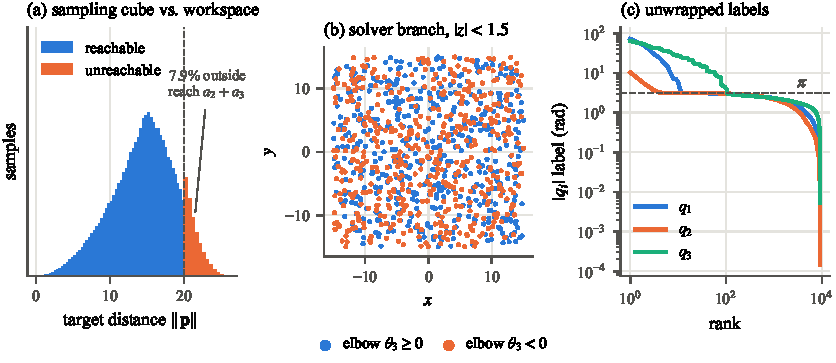
\includegraphics[width=\textwidth]{figures/fig_dataset.pdf}
\caption{Dataset pathologies (RRR). \textbf{(a)} Distribution of $\|\p\|$ for targets drawn uniformly from $[-15,15]^3$. Everything beyond the reach $a_2{+}a_3{=}20$ (7.9\%) is unsolvable, which explains the 8.2\% failure rate. \textbf{(b)} Elbow branch of the solver's label for dataset targets in the slab $|z|<1.5$. Neighbouring targets frequently receive solutions on different branches. \textbf{(c)} Sorted absolute joint labels on log axes. A tail of labels exceeds $\pi$ by up to $23\times$ because the solver does not wrap angles.}
\label{fig:dataset}
\end{figure*}

\subsection{The labels are not a well-posed regression target}
\label{sec:audit-labels}

\finding{2} \emph{The solver's branch choice is spatially incoherent.} Classifying each label by \cref{eq:ik-rrr}, the shoulder is ``front'' ($\sigma_s{=}{+}1$) for 81.4\% of samples, and the elbow splits 49.7\% / 50.3\%. Branch membership is not a smooth function of $\p$. For a held-out target, its nearest training target (median distance 0.84~LU, i.e.\ 4\% of the reach) lies on the same full branch only 66.0\% of the time: 74.5\% for the elbow alone and 86.2\% for the shoulder alone (\cref{fig:dataset}b). Starting every solve from $\q_0=\mathbf{0}$ yields a fixed but fragmented partition of the workspace into basins of attraction. A regressor must either memorise this partition, at the cost of poor generalisation, or average across it.

\finding{3} \emph{Labels are unwrapped.} 117 samples (1.27\%) contain a joint value outside $(-\pi,\pi]$, up to $q_1=-71.9$ and $q_3=63.8$~rad (\cref{fig:dataset}c). For MAE or MSE training, these points sit 10--70 radians away from geometrically identical labels.

Our LM replica reproduces the branch statistics closely: shoulder front 80.7\% vs.\ 81.4\% in the original data, elbow-up 50.6\% vs.\ 49.7\%. However, it unwraps angles far more often (66\% of solutions). We attribute this to step-control details of the specific toolbox release, which we cannot run. Our conclusions use the original labels wherever possible and use the replica only for failure and convergence statistics, which it matches.

\subsection{The RPP sampler draws a Cartesian coordinate from an angle range}
\label{sec:audit-rpp}

\finding{4} In \code{gen\_rpp.m}, the first input coordinate is sampled between \code{deg2rad(0)} and \code{deg2rad(360)}, so $x\in[0,2\pi]$ while $y,z\in[5,200]$. The earlier \code{train\_rpp.csv} used $x\in[0,360]$. This looks like a conflation of the target's $x$ coordinate with the base angle $\theta_1$. The effect on coverage is drastic: training targets lie in a slab $6.3$~LU thick, so the base angle spans only $\theta_1\in[-49.4^\circ,0^\circ]$, 13.7\% of the full rotation (\cref{fig:rpp}b). The resulting \code{model8000\_rpp\_rad} is accurate in-distribution (median task error 2.1~LU on a $\sim$200-LU workspace). But it degrades linearly as soon as $x$ leaves the slab (\cref{fig:rpp}a). On the input suggested in the RPP scripts, $[200,200,100]$, it returns $\hat\q=[0.087, 46.1, 175.0]$ against the exact $[-0.785, 95.0, 282.8]$, an error of 222~LU. For the earlier $x\in[0,360]$ data, our replica fails on 29.7\% of targets, against 28.8\% in the original file. All RPP labels are consistent with \cref{eq:fk-rpp} to within 0.13~LU.

\begin{figure*}[t]
\centering
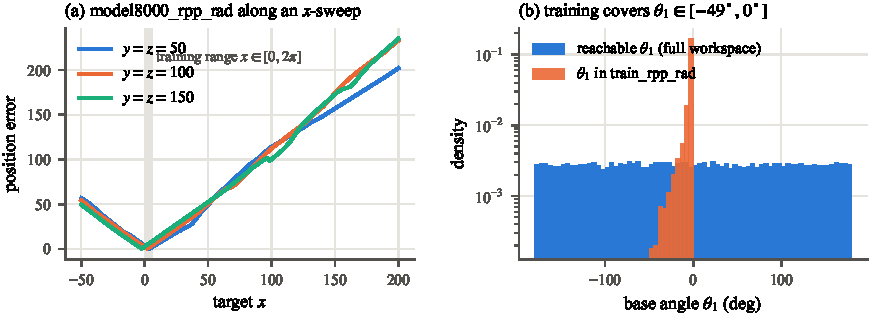
\includegraphics[width=\textwidth]{figures/fig_rpp.pdf}
\caption{RPP arm. \textbf{(a)} Task-space error of the original RPP network along $x$-sweeps at three heights. The shaded band is the training range of $x$, created by sampling $x$ from an angle interval. \textbf{(b)} Base angles covered by the training set (orange) versus the full reachable range (blue, log scale).}
\label{fig:rpp}
\end{figure*}

\subsection{What Keras's default accuracy measures}
\label{sec:audit-metric}

\finding{5} With \code{metrics=['accuracy']}, a three-unit output, and a non-cross-entropy loss, Keras resolves ``accuracy'' to \emph{categorical} accuracy,
\[
\mathrm{acc} = \frac1N\sum_n \mathbb{1}\big[\arg\max_j \hat q_{n,j} = \arg\max_j q_{n,j}\big].
\]
This only checks whether the \emph{largest of the three joint values} is in the same position. On its test split, \code{model20000\_rrr} scores 74.1\%; on the training split, 97.3\%. The metric is uninformative in both directions (\cref{tab:models}). The RPP model from the $x\in[0,360]$ data scores 91.4\% while its median position error is 148~LU, because its argmax is almost always $d_3$ (majority-class rate 81.0\%). Conversely, it could not distinguish a sub-millimetre solver from one that is off by $10^\circ$ in every joint.

\subsection{Worked example}
\label{sec:audit-provenance}

For $\p=[1,4,9]^\top$ ($\|\p\|=9.90$), the four exact solutions are listed in \cref{tab:case}. Any converged position-only solver must return one of them modulo $2\pi$. Our LM replica, started at $\mathbf{0}$, returns the $(+,+)$ branch $[75.96^\circ, 5.05^\circ, 120.66^\circ]$ after 13 iterations, modulo $2\pi$, but in unwrapped form. The baseline \code{model20000\_rrr} predicts $[78.77^\circ, 4.38^\circ, 121.21^\circ]$, on the same branch. It deviates from the exact solution by $(2.81^\circ, 0.67^\circ, 0.55^\circ)$, and its end effector lands 0.23~LU (2.3\% of $\|\p\|$) from the target. This target is representative of the median case. The tail of the error distribution (\cref{sec:reeval}) is dominated by targets on which the network switches branch.

\begin{table*}[t]
\centering
\small
\caption{Solutions for the example target $\p=[1,4,9]^\top$.}
\label{tab:case}
\begin{tabular}{lccc}
\toprule
Source & $(\theta_1,\theta_2,\theta_3)$ [deg] & $\FK(\q)$ & $\|\FK(\q)-\p\|$ \\
\midrule
Exact, $(\sigma_s,\sigma_e)=(+,+)$ & $(75.96,\ 5.05,\ 120.66)$ & $(1, 4, 9)$ & 0 \\
Exact, $(+,-)$ & $(75.96,\ 125.72,\ -120.66)$ & $(1, 4, 9)$ & 0 \\
Exact, $(-,+)$ & $(-104.04,\ 54.28,\ 120.66)$ & $(1, 4, 9)$ & 0 \\
Exact, $(-,-)$ & $(-104.04,\ 174.95,\ -120.66)$ & $(1, 4, 9)$ & 0 \\
LM replica from $\mathbf{0}$ (13 it.) & $(75.96,\ -354.95,\ 840.66)$ & $(1, 4, 9)$ & $<10^{-10}$ \\
\midrule
\code{model20000\_rrr} & $(78.77,\ 4.38,\ 121.21)$ & $(0.81, 4.07, 8.90)$ & 0.23 \\
\bottomrule
\end{tabular}
\end{table*}

\section{Task-Space Evaluation of the Baseline Models}
\label{sec:reeval}

\Cref{tab:models} evaluates all original models on their own (recovered) splits. Three points stand out.

\begin{table*}[t]
\centering
\small
\setlength{\tabcolsep}{4pt}
\caption{Original models on their recovered train/test splits. ``Keras acc.'' is Keras's default \code{'accuracy'} metric (\cref{sec:audit-metric}). ``Maj.'' is the categorical accuracy of always predicting the most frequent argmax index on the test split. Joint MAE uses wrapped differences. Task-space errors are in LU (RRR reach 20; RPP workspace $\sim$200). The last column is the share of targets with error $<1$~LU.}
\label{tab:models}
\begin{tabular}{lllrrcrrrr}
\toprule
Model & Arm & Split & Keras acc. & Maj. & Joint MAE [deg] & \multicolumn{3}{c}{Task-space error [LU]} & $<1$~LU \\
\cmidrule(lr){7-9}
 & & & [\%] & [\%] & $(q_1,q_2,q_3)$ & median & mean & p95 & [\%] \\
\midrule
\tabinput{tables/tab_models.tex}
\bottomrule
\end{tabular}
\end{table*}

\paragraph{Overfitting to the branch partition}
On its training split, \code{model20000\_rrr} has a wrapped joint MAE of $4$--$5^\circ$ and a median task error of 0.50~LU. On held-out targets, the joint MAE rises to $27$--$33^\circ$, and the mean task error more than doubles (0.85 to 2.19~LU). The test median is 0.78~LU (3.9\% of the reach), and the tail is heavy: the 95th percentile is 10.9~LU, more than half the reach, and only 0.5\% of test targets are within 0.1~LU (\cref{fig:rrr-error}a). The joint-space errors far exceed what the task-space errors would suggest, which is a signature of branch switching. The network lands on the label's branch for 68.8\% of test targets, with a median error of 0.60~LU; elsewhere the median error is 1.51~LU and the 95th percentile is 19.7~LU. The 26 test targets with unwrapped labels have a median error of 6.6~LU. Training longer (10k$\to$20k epochs) lowers the held-out median from 0.96 to 0.78~LU and the 95th percentile from 14.0 to 10.9~LU, while the train/test gap widens.

\paragraph{Geometry of the errors}
The median error is highest for targets near the origin (\cref{fig:rrr-error}b), where the folded-elbow singularity makes $\theta_2$ and $\theta_3$ ill-defined. It is also mildly elevated near the $z$-axis, where $\theta_1$ is undefined. A constant predictor (the mean training label) has a median error of 23.2~LU, so the network clearly learns most of the map. The question is whether the residual matters for the application, and \cref{tab:models} shows that it usually does.

\paragraph{The RPP models}
\code{model8000\_rpp\_rad} is the best-behaved model in the repository in-distribution: its $\theta_1$ error is $1.5^\circ$ and its median position error is 2.1~LU. This is expected, because the RPP inverse is single-valued and smooth on its training slab. Its failure is entirely one of coverage (\cref{sec:audit-rpp}). \code{model8000\_rpp} (data with $x\in[0,360]$) never learned a useful map: its median error is 148~LU, despite a Keras accuracy of 91.4\%.

\begin{figure*}[t]
\centering
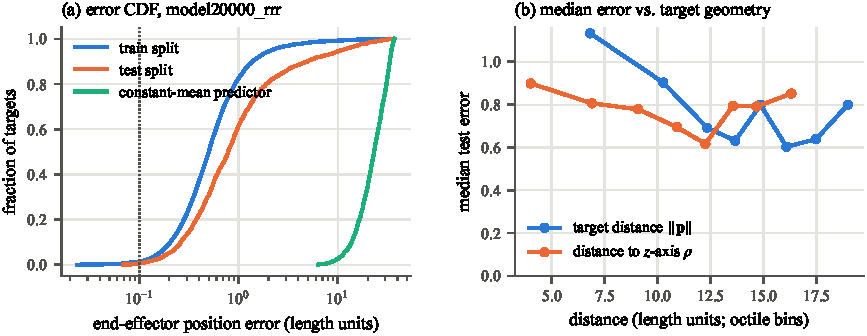
\includegraphics[width=\textwidth]{figures/fig_rrr_error.pdf}
\caption{Original \code{model20000\_rrr}. \textbf{(a)} Empirical CDF of task-space error on the training and test splits, together with a constant-mean predictor. The dotted line marks 0.1~LU. \textbf{(b)} Median test error in octile bins of target distance $\|\p\|$ and of distance to the $z$-axis $\rho$. Error peaks near the folded-elbow singularity at the origin.}
\label{fig:rrr-error}
\end{figure*}

\section{Controlled Study: What Makes Solver-Supervised IK Work?}
\label{sec:study}

The analysis identifies several suspects: inconsistent branches, unwrapped angles, the loss, and the output parameterisation. To separate their effects, we train identical networks on \emph{identical inputs}, namely the 7{,}344 training targets of the original RRR split, and vary one factor at a time. The RRR arm admits an exact, enumerable solution set (\cref{eq:ik-rrr}), so the label for each regime can be generated exactly.

\paragraph{Setup}
The five label regimes are:
\begin{itemize}
\item the solver's labels as generated;
\item the same labels wrapped to $(-\pi,\pi]$;
\item exact closed-form labels with a branch drawn uniformly at random per sample, i.e.\ maximal multiplicity;
\item exact labels on one consistent branch, $(\sigma_s,\sigma_e)=(+,+)$, with angle outputs;
\item the same consistent labels with a $(\cos q_i,\sin q_i)$ output head, decoded with $\atantwo$.
\end{itemize}
Each regime is trained with an L1 (MAE, as in the original) and an L2 (MSE) loss, three seeds each. The network is an MLP with three hidden layers of 256 ReLU units and fixed input scaling $\p/15$. Training uses Adam~\cite{kingma2015adam} at $\eta=2\times10^{-3}$ with cosine decay, 40k steps, and batch size 512, in PyTorch~\cite{paszke2019pytorch}. We evaluate on 20{,}000 fresh targets drawn uniformly from the reachable part of the original sampling cube. The original test split gives the same ranking.

\begin{table*}[t]
\centering
\small
\setlength{\tabcolsep}{4pt}
\caption{Controlled study on the RRR arm: identical inputs (7{,}344 targets), architecture, and optimiser; only the labels, loss, and output head change. The table reports task-space error on 20k fresh reachable targets (mean $\pm$ s.d.\ over 3 seeds; LU, reach $=20$). The ``$<$0.1'' columns give the share of targets with error below 0.1~LU, in \%.}
\label{tab:ablation}
\begin{tabular}{lrrrrrr}
\toprule
 & \multicolumn{3}{c}{L1 loss} & \multicolumn{3}{c}{L2 loss} \\
\cmidrule(lr){2-4}\cmidrule(lr){5-7}
Labels / output & median & p95 & $<$0.1 & median & p95 & $<$0.1 \\
\midrule
\tabinput{tables/tab_ablation.tex}
\bottomrule
\end{tabular}
\end{table*}

\paragraph{Results}
\Cref{tab:ablation} and \cref{fig:ablation}a show a clean separation into two groups that differ by almost two orders of magnitude. Every regime trained on solver labels or on mixed branches has a median error between 1.6 and 16~LU and a 95th percentile above 21~LU, i.e.\ beyond the arm's reach. Every regime trained on one consistent branch has a median below 0.075~LU and a 95th percentile below 0.17~LU. Within the two groups:
\begin{itemize}
\item \emph{Branch mixing is the dominant failure.} Drawing the branch at random per sample gives a median error of 14.4~LU (L1) and 16.0~LU (L2), 72--80\% of the reach, and not a single target below 0.5~LU. This is the averaging pathology of direct inverse modelling~\cite{jordan1992forward} in its pure form. The solver's labels sit between this extreme and a consistent labelling, as their partial spatial coherence (\cref{sec:audit-labels}) suggests.
\item \emph{The loss matters only when labels are multi-valued.} With solver labels, L1 is $3.2\times$ better than L2 at the median (1.94 vs.\ 6.27~LU). Under L1 the network tends to pick one mode of a locally bimodal target instead of averaging between modes, which probably explains why the original MAE choice worked at all. With consistent labels, the gap between the two losses mostly disappears.
\item \emph{Wrapping helps a little.} Wrapping the solver labels to $(-\pi,\pi]$ lowers the L1 median by 15\% (1.94 to 1.65~LU) but leaves the tail unchanged, because the 1.3\% of unwrapped labels is a minor problem next to branch switching.
\item \emph{A continuous output head is the last step.} With consistent labels, the $(\cos,\sin)$ head improves the L2 median from 0.074 to 0.042~LU and raises the share of targets below 0.1~LU from 72\% to 95\%. It removes the remaining discontinuity of $\theta_1$ and $\theta_2$ at $\pm\pi$~\cite{zhou2019continuity}.
\end{itemize}
Holding the inputs fixed, the best regime is therefore $43\times$ better at the median and $199\times$ better at the 95th percentile than the same network trained on the solver's labels (L1: 1.94 to 0.045~LU, and 21.9 to 0.110~LU). Our 40k-step budget does not reproduce the original model's absolute level on solver labels (median 1.94 vs.\ 0.76~LU, the latter after roughly $1.9\times10^5$ steps with a larger network). The ranking of the regimes, however, is unambiguous at this budget.

\begin{figure*}[t]
\centering
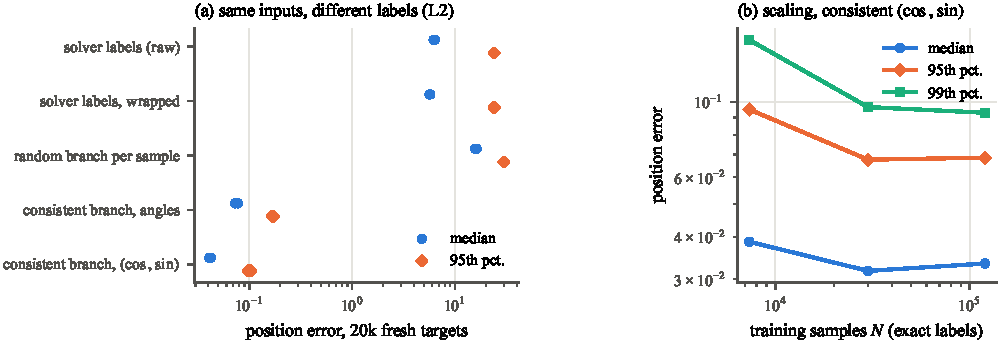
\includegraphics[width=\textwidth]{figures/fig_ablation.pdf}
\caption{\textbf{(a)} Controlled study (L2 loss): median and 95th-percentile task-space error on 20k fresh targets. The bars span three seeds. \textbf{(b)} Scaling the consistent $(\cos,\sin)$ model with exact labels drawn uniformly in the reachable cube; values are means over three seeds.}
\label{fig:ablation}
\end{figure*}

\paragraph{Scaling with exact labels}
With exact labels sampled uniformly in the reachable cube and a 60k-step budget (\cref{tab:scaling}, \cref{fig:ablation}b), the consistent $(\cos,\sin)$ network reaches a median error of 0.039~LU from the original 7{,}344 inputs and 0.032~LU from 30k samples. The 99th percentile falls from 0.15 to 0.10~LU, and 99.1\% of targets are within 0.1~LU. Quadrupling the data again to 120k gives no further gain (median 0.033~LU), so at this budget the error is limited by optimisation and capacity, not by data. Compared with the original \code{model20000\_rrr} on the same 20k fresh targets, the 30k-sample model is $24\times$ better at the median (0.763 to 0.032~LU), $177\times$ better at the 95th percentile (11.9 to 0.068~LU), and $252\times$ better at the 99th (24.3 to 0.097~LU). It does this with 42\% fewer parameters and without any solver in the data-generation loop.

\begin{table*}[t]
\centering
\small
\caption{Original model versus the consistent $(\cos,\sin)$ model trained on $N$ exact labels (60k steps), evaluated on the same 20k fresh reachable targets. Errors in LU.}
\label{tab:scaling}
\begin{tabular}{lcrrrr}
\toprule
Model & Seeds & median & p95 & p99 & $<$0.1~LU [\%] \\
\midrule
\tabinput{tables/tab_scaling.tex}
\bottomrule
\end{tabular}
\end{table*}

\paragraph{Learned warm starts}
A learned map can also serve as the initial guess of a numerical solver. This keeps the solver's accuracy and convergence check and uses the network only to choose where to start. \Cref{tab:hybrid} compares three initial guesses on 3{,}000 fresh reachable targets. From $\q_0=\mathbf{0}$, as in the original scripts, LM converges in 15.8 iterations on average, and only 39.5\% of its solutions land on the $(+,+)$ branch; the rest are scattered over the other three. A warm start from the original network cuts the iterations to 6.2, but the branch distribution is unchanged (39.7\%), because the network inherited the solver's incoherent branch choice. A warm start from the consistent network needs 4.5 iterations on average (95th percentile 5) and returns the $(+,+)$ branch for \emph{every} target. No initialisation produced a failure on reachable targets. In this hybrid scheme the learned model contributes branch selection and speed, while the solver guarantees accuracy.

\begin{table*}[t]
\centering
\small
\caption{LM (\code{ikine} replica) on 3{,}000 fresh reachable targets with different initial guesses. ``Target branch'' is the share of solutions on the $(+,+)$ branch. A consistent learned warm start makes the solver's output branch predictable.}
\label{tab:hybrid}
\begin{tabular}{lrrrrr}
\toprule
Initial guess & Fail & \multicolumn{3}{c}{LM iterations} & Target branch \\
\cmidrule(lr){3-5}
 & [\%] & mean & median & p95 & [\%] \\
\midrule
\tabinput{tables/tab_hybrid.tex}
\bottomrule
\end{tabular}
\end{table*}

\paragraph{Latency}
\Cref{tab:latency} reports wall-clock cost in Python/NumPy. The closed-form solution is the fastest method in both single-query (12.7~\textmu s) and batched (0.13~\textmu s per query) use, and it is exact. The original 233k-parameter MLP is $4\times$ slower than closed form for a single query and $23\times$ slower batched. The leaner consistent network is $1.4\times$ and $11\times$ slower, respectively. The LM replica from $\q_0=\mathbf{0}$ takes 358~\textmu s on a representative target, and 89~\textmu s from a learned warm start. Including the 18~\textmu s network evaluation, this is a $3.3\times$ speed-up. A learned model is thus not a faster solver for an arm that has a closed form. It \emph{is} a cheap way to accelerate and steer an iterative solver, which is the regime that matters for arms without one.

\begin{table}[t]
\centering
\small
\caption{Wall-clock cost per IK query in Python/NumPy on an Apple M1 Pro CPU (single query: mean over 2{,}000 calls; batched: $10^4$ targets per call). Absolute values depend on the implementation; ratios are the informative quantity.}
\label{tab:latency}
\resizebox{\columnwidth}{!}{%
\begin{tabular}{lrr}
\toprule
Method & Single [\textmu s] & Batched [\textmu s/query] \\
\midrule
\tabinput{tables/tab_latency.tex}
\bottomrule
\end{tabular}}
\end{table}

\section{Discussion}
\label{sec:discussion}

\paragraph{What the baseline learns}
The baseline network learns a coarse approximation of the RRR inverse map: its median error is 3.9\% of the reach, far better than a constant predictor, and on a typical target it is within $3^\circ$ of an exact solution. Its accuracy is limited by its training labels rather than its capacity. The same network trained on consistent labels is two orders of magnitude more accurate (\cref{sec:study}). Each limitation of the baseline arises from a default that looks reasonable in isolation: Keras's \code{'accuracy'} metric, the solver's fixed initial guess, and its unwrapped output.

\paragraph{Where a learned IK model helps}
For the two arms studied here, a closed-form solver is exact and faster than any network (\cref{tab:latency}), so the learned model has no role \emph{as a solver}. Its value lies elsewhere. (i) Arms without closed-form IK (redundant, or with offset wrists) have no exact alternative. (ii) As a warm start, a consistent learned map fixes which branch the downstream solver returns, which a fixed initial guess cannot do (\cref{tab:hybrid}). (iii) Batched, differentiable inverse maps can be embedded in planning or learning loops. In all three cases, the lessons below apply unchanged.

\paragraph{A checklist for solver-supervised IK learning}
\begin{enumerate}[label=\textbf{C\arabic*.}, leftmargin=*]
\item \textbf{Sample where solutions exist.} Sample joint space and apply $\FK$, or reject targets outside the workspace. Do not interpret solver failures as singularities without checking reachability.
\item \textbf{Make the label a function.} Either fix a branch (a canonical selection rule, or a consistent warm start) or model the multiplicity explicitly~\cite{bishop1994mixture,ames2022ikflow}. Never mix branches from basin-dependent solver output.
\item \textbf{Canonicalise angles} and prefer a continuous output head such as $(\cos,\sin)$~\cite{zhou2019continuity}.
\item \textbf{Measure in task space.} Report $\|\FK(\hat\q)-\p\|$ with medians \emph{and} tails, plus wrapped joint errors. Never use a classification ``accuracy'' for regression.
\item \textbf{Check ranges against units.} The inputs are Cartesian coordinates, not angles. Plot the training distribution against the intended workspace.
\item \textbf{Keep held-out data held out}, including for qualitative figures, and state which split every plot comes from.
\item \textbf{Time it} against the strongest available baseline, including closed form when it exists.
\end{enumerate}

\paragraph{Limitations}
MATLAB was not available to us, so the solver statistics come from a re-implementation. It matches the original data's failure rate and branch distribution, but not its angle-unwrapping frequency. All findings about the original models use the original weights and data. The controlled study uses a single small architecture and 3-DOF position IK. Redundant arms and full 6-DOF poses would strengthen the conclusions about warm starts. Latency is measured in Python and is only indicative.

\section{Conclusion}
\label{sec:conclusion}

We presented and analysed a solver-supervised neural IK pipeline for two 3-DOF manipulators. Keras's default accuracy is an argmax-agreement score that does not measure IK quality. The solver's failures are workspace violations, its labels are branch-incoherent and unwrapped, and one generator sampled a Cartesian coordinate from an angle range. Measured in task space, the baseline RRR network reaches a median end-effector error of about 4\% of the reach, with a heavy tail. With the inputs held fixed, consistent exact labels and a continuous output head reduce the error by $43\times$ at the median and $199\times$ at the 95th percentile. Trained on 30k exact samples, a smaller network beats the baseline model by $24\times$ at the median and $177\times$ at the 95th percentile. Used as a warm start, a consistent learned map makes a numerical solver converge $3.5\times$ faster and always return the intended branch. The broader lesson is that, in learned IK, the label-generation procedure and the evaluation metric need as much scrutiny as the network itself.

\section*{Code and Data Availability}
The original project artifacts and the analysis code (\code{paper/code}: \code{audit.py}, \code{improved.py}, \code{figures.py}, \code{make\_tables.py}) regenerate every number, table, and figure in this report.

\section*{Acknowledgment}
The pipeline analysed here was built for Project~2 of MAE~547 (Modeling and Control of Robots) at Arizona State University, Fall 2021, by the author together with Rumitkumar Patel and Priyank Patel. The author thanks them for their work on the original artifacts. The analysis, re-evaluation, controlled study, and this report are the author's own subsequent work. The 2026 re-analysis was carried out with the assistance of an AI coding assistant; all results were produced by the released scripts, and the author takes full responsibility for the content.

\bibliographystyle{IEEEtran}
\bibliography{refs}

\appendices




\section{LM Solver Re-implementation}
\label{app:lm}

\begin{algorithm}[t]
\caption{Position-only LM IK (replica of RTB \code{SerialLink.ikine} as used)}
\label{alg:lm}
\begin{algorithmic}[1]
\Require target $\p^\star$, initial $\q_0$; $\lambda\gets0.1$, $\varepsilon=10^{-10}$, $I_{\max}=1000$, $R_{\max}=100$
\State $\q\gets\q_0$, $\mathbf e\gets\p^\star-\FK(\q)$, $k\gets0$, $r\gets0$
\Loop
  \State $k\gets k+1$; \textbf{if} $k>I_{\max}$ \textbf{return} \textsc{fail}
  \State \textbf{if} $\|\mathbf e\|<\varepsilon$ \textbf{return} $\q$
  \State $J\gets\partial\FK/\partial\q\,(\q)$;\quad $\Delta\q\gets(J^\top J+\lambda I)^{-1}J^\top\mathbf e$
  \If{$\|\p^\star-\FK(\q+\Delta\q)\|<\|\mathbf e\|$}
     \State $\q\gets\q+\Delta\q$, $\mathbf e\gets\p^\star-\FK(\q)$, $\lambda\gets\lambda/2$, $r\gets0$
  \Else
     \State $\lambda\gets2\lambda$, $r\gets r+1$; \textbf{if} $r>R_{\max}$ \textbf{return} \textsc{fail}
  \EndIf
\EndLoop
\end{algorithmic}
\end{algorithm}

With a position-only mask, the toolbox's end-effector-frame error and Jacobian give the same step as the world-frame form above, since the rotation cancels in $J^\top W\mathbf e$. Rejected steps count towards the iteration limit, as in the toolbox loop.

\section{Reproduction}
\label{app:repro}

{\footnotesize
\begin{verbatim}
pip install h5py numpy pandas scipy \
            scikit-learn matplotlib torch
cd paper/code
python audit.py      # Part I  (~30 s)
python improved.py   # Part II (~45 min CPU)
python figures.py; python make_tables.py
cd .. && tectonic main.tex
\end{verbatim}}
No TensorFlow installation is needed: Keras weights are read directly from HDF5 and evaluated in NumPy.

\end{document}
